\documentclass{beamer}
\usepackage{graphicx}
\usepackage{caption}
\usepackage{float}
\usepackage{multicol}
\usepackage[utf8]{inputenc}

\title{Mineração de dados aplicada à dados de evento no futebol}
\author{Luis Felipe Ramos \and Igor Lacerda Faria da Silva \and Matheus Tiago Pimenta de Souza}
\date{2024-07-28}

\captionsetup[figure]{labelformat=empty}% redefines the caption setup of the figures environment in the beamer class.

\begin{document}

\frame{\titlepage}

\begin{frame}
\frametitle{Uso de ciência de dados aplicada ao esporte}

\begin{columns}
\begin{column}{0.5\textwidth}
\centering
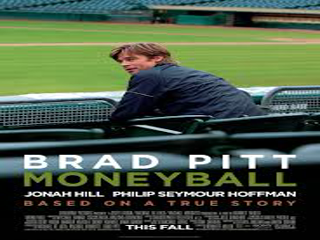
\includegraphics[width=\linewidth]{moneyball.png}
\captionof{figure}{Moneyball (2011)}
\end{column}
\begin{column}{0.5\textwidth}
\centering
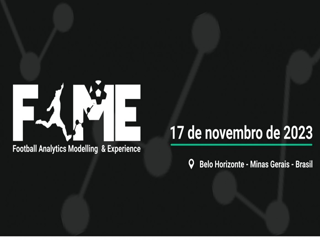
\includegraphics[width=\linewidth]{fame.png}
\captionof{figure}{FAME}
\end{column}
\end{columns}
\end{frame}

\begin{frame}
\frametitle{Dados de súmula no futebol}
\begin{figure}[H]
\centering
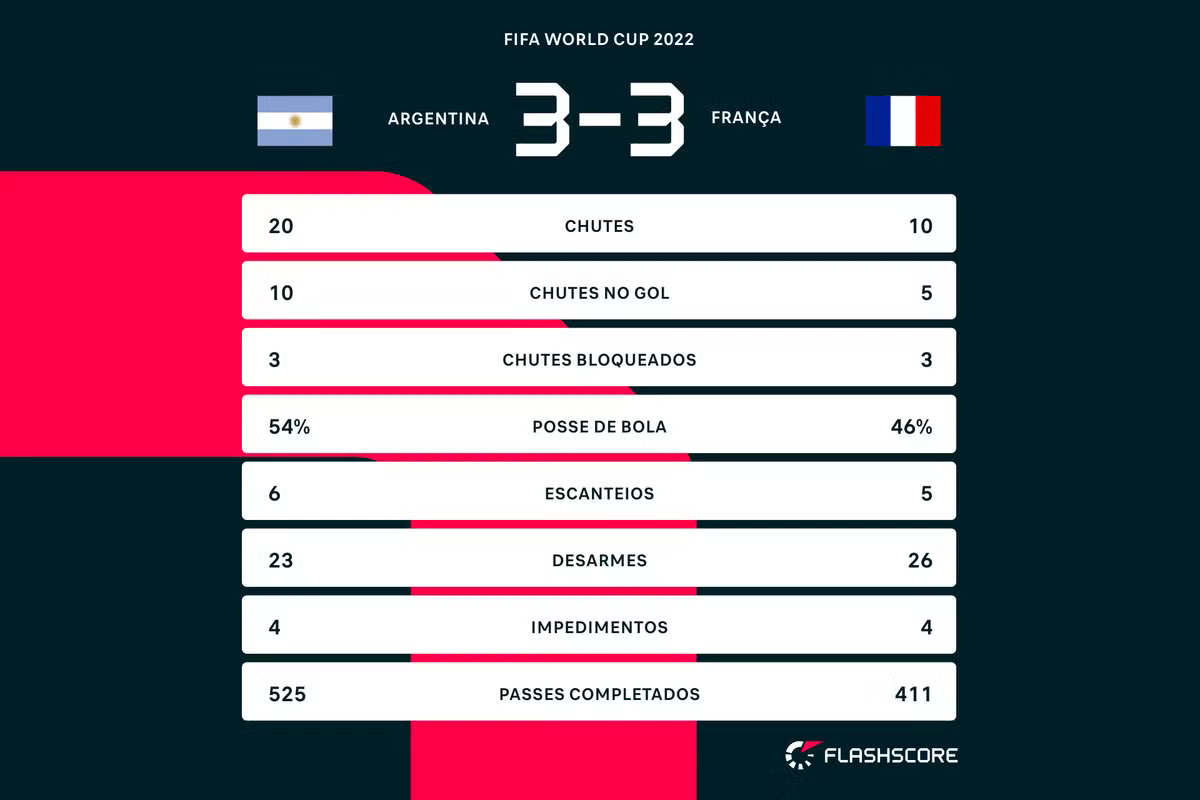
\includegraphics[width=\linewidth]{copa.jpg}
\caption{Estatísticas da final da Copa do Mundo de 2022}
\end{figure}
\end{frame}

\begin{frame}
\frametitle{Dados de evento}
\begin{figure}[H]
\centering
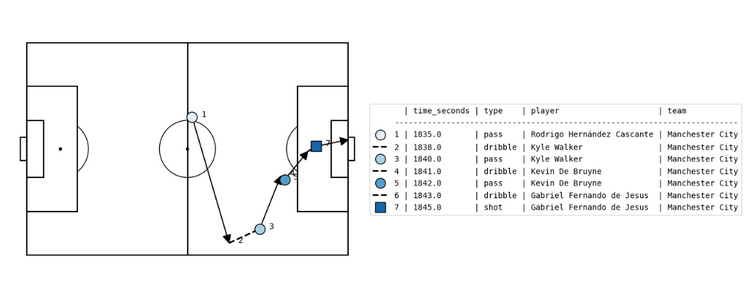
\includegraphics[width=\linewidth]{eventdatacity.png}
\caption{Jogada do Manchester City}
\end{figure}
\end{frame}

\begin{frame}
\frametitle{SPADL}
\begin{table}[H]
\centering
\begin{tabular}{|l|l|}
\hline
\textbf{Atributo} & \textbf{Descrição} \\
\hline
game\_id & O ID do jogo no qual a ação foi realizada \\
\hline
period\_id & O ID do período do jogo no qual a ação foi realizada \\
\hline
seconds & O tempo de início da ação \\
\hline
player & O jogador que realizou a ação \\
\hline
team & O time do jogador \\
\hline
start\_x & A localização x onde a ação começou \\
\hline
start\_y & A localização y onde a ação começou \\
\hline
end\_x & A localização x onde a ação terminou \\
\hline
end\_y & A localização y onde a ação terminou \\
\hline
action\_type & O tipo de ação (por exemplo, passe, chute, drible) \\
\hline
result & O resultado da ação (por exemplo, sucesso ou falha) \\
\hline
bodypart & A parte do corpo do jogador usada para a ação \\
\hline
\end{tabular}
\caption{Descrição dos dados no formato SPADL}
\end{table}
\end{frame}

\begin{frame}
    \frametitle{Distribuição dos tipos de ações}
\begin{figure}[H]
\centering
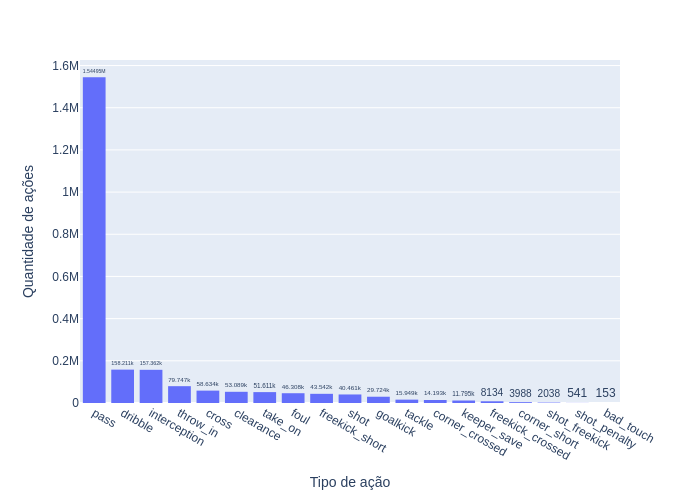
\includegraphics[width=\linewidth]{../report/images/action_distribution.png}
\end{figure}
\end{frame}

\begin{frame}
    \frametitle{Mapa de calor dos gols}
\begin{figure}[H]
\centering
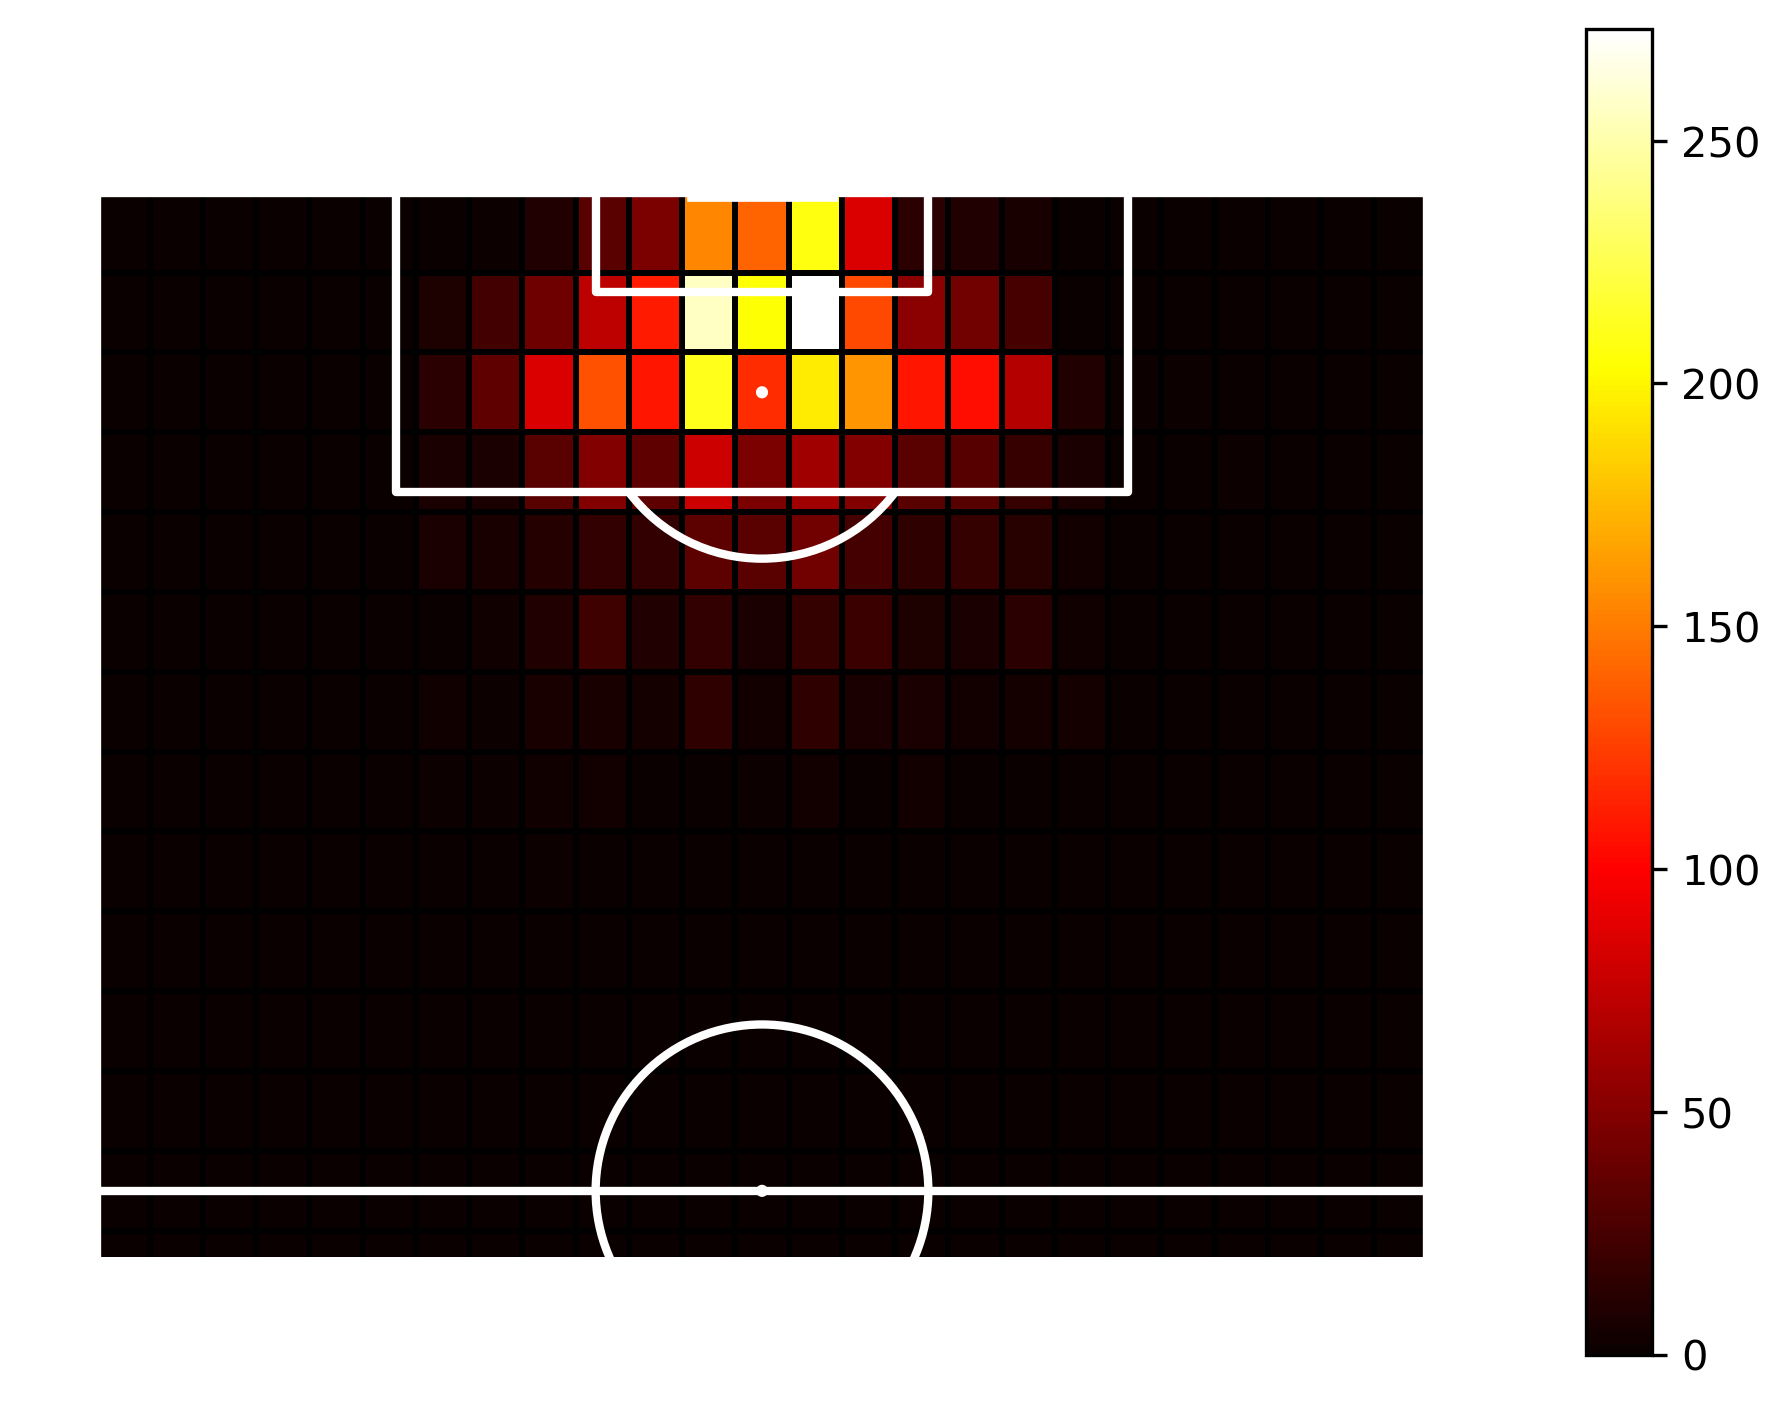
\includegraphics[width=\linewidth]{../report/images/goal_position_heatmap.png}
\end{figure}
\end{frame}

\begin{frame}
\frametitle{Objetivos}
\framesubtitle{Descoberta de subgrupos}
\begin{itemize}
    \item Trabalho motivador: \textit{Subgroup Discovery in Soccer Data}
    \item Reproduzir os experimentos do artigo e experimentar com novos algoritmos de SD
\end{itemize}
\end{frame}

\begin{frame}
\frametitle{Objetivos}
\framesubtitle{Mineração de sequências}
\begin{itemize}
    \item Trabalho motivador: \textit{Supervised sequential pattern mining of event sequences in sport to identify important patterns of play: An application to rugby union}
    \item Aplicar as ideias em sequências de jogadas de futebol
\end{itemize}
\end{frame}

\begin{frame}
\frametitle{Gols Esperados (xG)}
\begin{itemize}
    \item Métrica de cálculo de probabilidade de gol
    \item Diferentes \textit{features} podem ser utilizadas:
    \begin{itemize}
        \item Distância para o gol
        \item Ângulo de chute
    \end{itemize}
\end{itemize}
\begin{figure}[H]
\centering
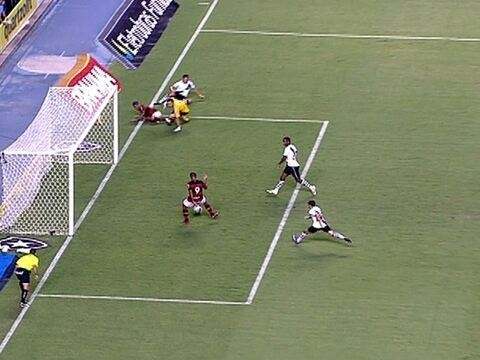
\includegraphics[width=\linewidth]{deivid.jpg}
\end{figure}
\end{frame}

\begin{frame}
\frametitle{VAEP}
\begin{itemize}
    \item Ações valem mais do que apenas gols
    \item O quanto cada jogada contribui para o aumento da chance de gol e diminiuição da chance de tomar gol?
\end{itemize}
\begin{figure}[H]
\centering
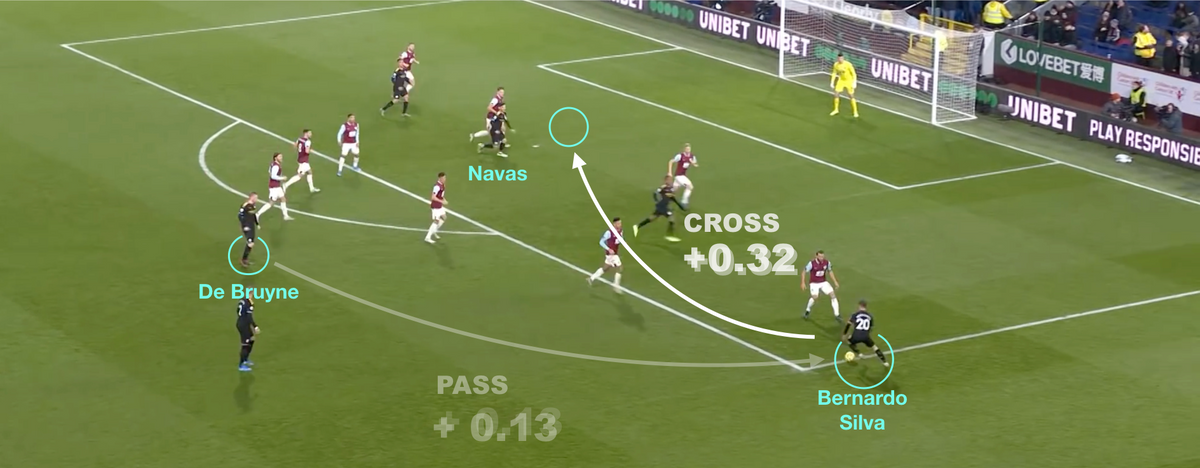
\includegraphics[width=\linewidth]{vaep.png}
\end{figure}
\end{frame}

\begin{frame}
\frametitle{Descoberta de subgrupos}
-res
\end{frame}

\begin{frame}
\frametitle{Mineração de sequências}
-res
\end{frame}

\begin{frame}
\frametitle{Fim}
\begin{itemize}
    \item Perguntas, comentários, etc 
\end{itemize}
\end{frame}

\end{document}

